% !TeX encoding = UTF-8
% !TeX root = ../main.tex

%% ------------------------------------------------------------------------
%% Copyright (C) 2021 SJTUG
%% 
%% SJTUBeamer Example Document by SJTUG
%% 
%% SJTUBeamer Example Document is licensed under a
%% Creative Commons Attribution-NonCommercial-ShareAlike 4.0 International License.
%% 
%% You should have received a copy of the license along with this
%% work. If not, see <http://creativecommons.org/licenses/by-nc-sa/4.0/>.
%% -----------------------------------------------------------------------

\section{学位论文排版}
\subsection{\SJTUThesis 上海交通大学学位论文模板}

\begin{frame}{\SJTUThesis}
  \framesubtitle{上海交通大学学位论文 \LaTeX{} 模板}
  \begin{itemize}
    \item 最早由韦建文于 2009 年 11 月发布 0.1a 版,2018 年起由 SJTUG 接手维护
    \item 最新版:\SJTUThesisVersion{} (\SJTUThesisDate)
    \item 支持本科、硕士、博士学位论文以及课程论文的排版
  \end{itemize}
  \begin{figure}[htbp]
    \centering
    
\includegraphics[height=.4\textheight]{sjtuthesis-bachelor-crop.pdf}\hspace{6pt}
    
\includegraphics[height=.4\textheight]{sjtuthesis-master-crop.pdf}\hspace{6pt}
    
\includegraphics[height=.4\textheight]{sjtuthesis-doctor-crop.pdf}\hspace{6pt}
    
\includegraphics[height=.4\textheight]{sjtuthesis-course-crop.pdf}
  \end{figure}
\end{frame}

\begin{frame}[fragile]{获取\SJTUThesis{}}
  \begin{columns}
    \begin{column}{.65\textwidth}
      \begin{itemize}
        \item 下载最新版(推荐)
              \begin{itemize}
                \item GitHub Releases \link{https://github.com/sjtug/SJTUThesis/releases}
                \item OverLeaf \link{https://www.overleaf.com/latex/templates/sjtuthesis-latex-thesis-template-for-shanghai-jiao-tong-university/mkdwbyjbtfgg?r=b3b31f49&rm=d&rs=b}
              \end{itemize}
        \item 下载最新开发版(高级 / 想尝鲜 / 着急的用户)
              \begin{itemize}
                \item \url{https://github.com/sjtug/SJTUThesis}
                \item 切换到 |develop| 分支,点右边栏
                      \href{https://github.com/sjtug/SJTUThesis/archive/dev.zip}%
                      {Download ZIP} 按钮
              \end{itemize}
        \item 编译
              \begin{itemize}
                \item 解压缩看文档 |README.md|
                \item Windows: 双击 |Compile.bat| 脚本编译
                \item Linux \& macOS: 使用 |Makefile|
                \item 使用 |latexmk -xelatex main|
              \end{itemize}
      \end{itemize}
    \end{column}
    \begin{column}{.25\textwidth}
      \begin{figure}[htbp]
        \centering
        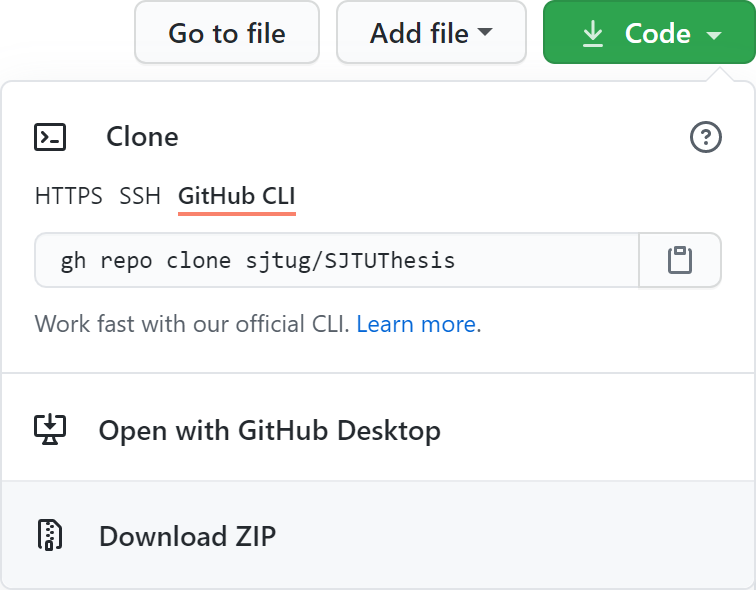
\includegraphics[width=\textwidth]{sjtuthesis-download.png}
      \end{figure}
      \vfill
    \end{column}
  \end{columns}
\end{frame}

\begin{frame}[fragile]{模板选项}
  \begin{description}
    \item[type] 指定论文类型(本科/硕士/博士/课程)
      \begin{lstlisting}[basicstyle=\ttfamily]
\documentclass[type=bachelor]{sjtuthesis}
  \end{lstlisting}
    \item[review] 开启盲审模式
      \begin{lstlisting}[basicstyle=\ttfamily]
\documentclass[type=master,review]{sjtuthesis}
  \end{lstlisting}
    \item[fontset] 指定字体(推荐使用 |windows|)
      \begin{lstlisting}[basicstyle=\ttfamily]
\documentclass[type=doctor,fontset=windows]{sjtuthesis}
  \end{lstlisting}
  \end{description}
\end{frame}

\begin{frame}[fragile]{模板设置}
  使用 |\sjtusetup| 命令指定论文各类设置:
  \begin{lstlisting}
\sjtusetup{
  info = {
    title             = {上海交通大学学位论文 \LaTeX{} 模板示例文档},
    title*            = {A Sample for \LaTeX-based SJTU Thesis Template},
    author            = {某\quad{}某},
    author*           = {Mo Mo},
  },
  style = {
    header-logo-color = red,
  },
  name = {
    publications      = {攻读学位期间完成的论文},
  },
}
  \end{lstlisting}
\end{frame}

\begin{frame}[fragile]{信息录入}
  |info| 域完成论文基本信息录入
  \begin{table}[h]
    \centering
    \footnotesize
    \begin{tabular}{lll} \toprule
      命令作用     & 中文对应选项                      & 英文对应选项      \\ \midrule
      论文标题     & |title|                           & |title*|          \\
      关键字列表   & |keywords|                        & |keywords*|       \\
      作者姓名     & |author|                          & |author*|         \\
      申请学位名称 & |degree|                          & |degree*|         \\
      院系名称     & |department|                      & |department*|     \\
      专业名称     & |major|                           & |major*|          \\
      导师         & |supervisor|                      & |supervisor*|     \\
      副导师       & |assisupervisor|                  & |assisupervisor*| \\
      日期         & \multicolumn{2}{c}{\texttt{date}}                     \\
      学号         & \multicolumn{2}{c}{\texttt{id}}                       \\ \bottomrule
    \end{tabular}
  \end{table}
\end{frame}

\begin{frame}[fragile]{数学}
  \begin{itemize}
    \item 公式示例:\nolinkurl{contents/math_and_citations.tex}
    \item \SJTUThesis{} 定义了常用的数学环境(需要手工引入 |amsthm| 宏包):
          \begin{table}[h]
            \centering
            \footnotesize
            \begin{tabular}{*{7}{l}}\toprule
              assumption & axiom   & conjecture & corollary   & definition & example  & exercise \\
              假设       & 公理    & 猜想       & 推论        & 定义       & 例       & 练习     \\\midrule
              lemma      & problem & proof      & proposition & remark     & solution & theorem  \\
              引理       & 问题    & 证明       & 命题        & 注         & 解       & 定理     \\\bottomrule
            \end{tabular}
          \end{table}
    \item \SJTUThesis{} 使用 \pkg{unicode-math} 进行数学输入(\ref{frame:unicode-math} 页),注意与传统方式的区别
  \end{itemize}
\end{frame}

\begin{frame}[fragile]{参考文献}
  \begin{itemize}
    \item 建议自动生成
          \begin{itemize}
            \item \LaTeX 引擎自身不能处理参考文献,需要借助外部程序!
          \end{itemize}
    \item 传统方法:\BibTeX 后端
          \begin{itemize}
            \item 控制文献、引用样式:\pkg{natbib} 宏包
            \item 国标样式:\pkg{gbt7714} 宏包 \link{https://mirrors.sjtug.sjtu.edu.cn/ctan/biblio/bibtex/contrib/gbt7714/gbt7714.pdf}
          \end{itemize}
    \item 现代方法:|biber| 后端 + \pkg{biblatex} 宏包
          \begin{itemize}
            \item 国标样式:\pkg{biblatex-gbt7714-2015} 宏包 \link{https://mirrors.sjtug.sjtu.edu.cn/ctan/macros/latex/contrib/biblatex-contrib/biblatex-gb7714-2015/biblatex-gb7714-2015.pdf}
          \end{itemize}
    \item 需要多轮编译——再次推荐 latexmk
  \end{itemize}
\end{frame}

\begin{frame}[fragile]{参考文献(续)}
  \begin{itemize}
    \item 生成 |.bib| 数据库
          \begin{itemize}
            \item Google Scholar 可直接复制或者批量导出
            \item 用 Zotero、Jabref 等文献管理软件生成
          \end{itemize}
    \item 两种引用模式:
          \begin{itemize}
            \item 上标模式:如“在许多文献\textsuperscript{[12-13]}中……”
                  \begin{lstlisting}[basicstyle=\ttfamily]
    \cite{key12, key13}
          \end{lstlisting}
            \item 正文模式:如“文献~[14] 证明了……”
                  \begin{lstlisting}[basicstyle=\ttfamily]
    \parencite{key14}
          \end{lstlisting}
          \end{itemize}
  \end{itemize}
\end{frame}

\begin{frame}[fragile]{\SJTUThesis 问题}
  \begin{itemize}
    \item 常见问题
          \begin{itemize}
            \item 参考文献列表出错、缺少字体、无法编译、格式不对……
            \item 阅读模板文档 |sjtuthesis.pdf| 和 SJTUThesis 示例文档代码
            \item 查看 FAQ \link{https://github.com/sjtug/SJTUThesis/wiki/常见问题}
          \end{itemize}
    \item 主动提问
          \begin{itemize}
            \item GitHub Issues 提问:\link{https://github.com/sjtug/SJTUThesis/issues}
          \end{itemize}
  \end{itemize}
\end{frame}
